% !TeX root = ../Thesis.tex

\chapter{Theorie}\label{ch:Theory}
%This chapter should introduce to the theoretical background of your thesis. Any (already existing) method you use to obtain the results later should be introduced and explained. The mathematics needed to understand the possibly new methods in the next chapter is also part of this chapter. 

%https://www.ebi.ac.uk/biostudies/BioImages/studies/S-BIAD1518?query=3D%20nuclei%20segmentation

\section{Überblick}
Im nachfolgenden Kapitel wird der theoretische Hintergrund der vorliegenden Thesis behandelt. 
Hierzu werden sowohl für die Arbeit relevante Methoden als auch die Literatur verwandter Projekte und Studien zum aktuellen Stand der Technik beleuchtet. 
Da die Arbeit im Kern die panoptische Segmentierung von Zelldaten behandelt werden hier Methoden zur Instanzsegmentierung und zu Klassifikation angeführt.
Die Methoden zu Instanzsegmentierung sind konzentriert auf \ac{ki}-Methoden, von klassischen Ansätzen wird abgesehen.
Für die Klassifikation wird von grundlegenden Erklärungen von Deep-Learning-Methoden abgesehen und moderne Ansätze sowie relevante Methoden zur Visualisierung oder Optimierung von Klassifikatoren angeführt.
Um die Methoden in einem vergleichbaren und repoduzierbaren Aufbau zu demonstrieren werden außerdem Benchmark-Methoden beleuchtet.
Dem theoretischen Hintergrund wird der Neuheitswert der Arbeit gegenübergestellt, um den Beitrag des vorliegenden Projekts zur Forschung zu verdeutlichen.

\section{Methoden}
\subsection{Benchmark}
Um die Leistungsfähigkeit der Applikation, die im Rahmen der vorliegenden Thesis erstellt wird, zu prüfen, sind umfangreiche Datensätze notwendig. 
Für jede isolierbare Aufgabe muss ein Datensatz gewählt werden, der Annotationen entsprechend dieser Aufgabe mitbringt.
Die Herausforderung bei der Auswahl eines Datensatzes ist, dass die darin enthaltenen Daten (Quelldaten) den Daten, für die die Anwendung entworfen wird (Zieldaten), \textit{ähnlich} sein müssen.
So wird sichergestellt, dass sich die auf den Quelldaten gemessene Qualität der Anwendung sinnvoll auf die Zieldaten übertragen lässt \cite{ganin2015domain_big}.
Der Begriff \textit{Ähnlichkeit} ist mehrdeutig und das Definieren von Merkmalen in Daten, die das Messen von \textit{Ähnlichkeit} ermöglichen, ist anspruchsvoll.
Metriken, die als Maß für \textit{Ähnlichkeit} genutzt werden müssen, müssen maßgeschneidert zur Anwendung passen und sind bereits breit erforscht \cite{zhu2020domain_similarity, koohi2018similarity, cai2009similarity}.
Daten können mithilfe passender Metriken \textit{Ähnlichkeits-}gruppen, sogenannten \textit{Domänen}, zugeordnet werden \cite{yuan2005domainsimilarity}.
Beispiele für Domänenunterschiede in biomedizinischen Bildaufnahmen sind verschiedene Farb-Marker, Aufnahmegeräte oder Zoom-Stufen. 
In Abb. \ref{fig:domains} sind Zellkerne in verschiedenen Darstellungen angebildet. \newline
%\newline Altes Bild (Katzen) ersetzt \newline
%\begin{figure}[htbp]
%    \centering
%    \includegraphics[width=0.18\textwidth]{Figures/Katze_0.jpg} \hfill
%    \includegraphics[width=0.24\textwidth]{Figures/Katze_1.jpg}\hfill
%    \includegraphics[width=0.24\textwidth]{Figures/Katze_3.jpg}\hfill
%    \includegraphics[width=0.24\textwidth]{Figures/Katze_2.jpg}
%    \caption{Vier Bilder der Klasse \textit{Katze} aus verschiedenen Bilddomänen. Von Links nach Rechts steigt der wahrgenommene Abstraktionsgrad \cite{jrfarm_katze, Egan_Katzen}.}
%    \label{fig:domains}
%\end{figure}
\begin{figure}[H]
    \centering
    \begin{subfigure}[c]{0.24\textwidth} 
        \includegraphics[width=\textwidth]{Figures/Cell_domain0.jpg}
        \caption{3D-Bildstapel mit verschiedenen Fluoreszenzmarkern, aufgenommen mit einem Leica TCS SP8 Konfokalmikroskop.}
    \end{subfigure} \hfill
    \begin{subfigure}[c]{0.24\textwidth}
        \includegraphics[width=\textwidth]{Figures/Cell_domain1.jpg}
        \caption{3D-SIM Superauflösungsmikroskopie mit DAPI-Färbung \cite{Schermelleh2008}.}
    \end{subfigure} \hfill
    \begin{subfigure}[c]{0.24\textwidth}
        \includegraphics[width=\textwidth]{Figures/Cell_domain2.jpg}
        \caption{Konfokale Fluoreszenzmikroskopie mit antikörperbasierten Farbstoffen \cite{Peng2015}.}
    \end{subfigure} \hfill
    \begin{subfigure}[c]{0.24\textwidth}
        \includegraphics[width=\textwidth]{Figures/Cell_domain3.jpg}
        \caption{Klassische Hellfeldmikroskopie \cite{Ali2012}.}
    \end{subfigure}
    \caption{Vier Aufnahmen von Zellen. Die Bilddomänen sind durch die verschiedenen Marker und Aufnahmetechniken klar zu unterscheiden \cite{Schermelleh2008, Peng2015, Ali2012}.}
    \label{fig:domains}
\end{figure}

Intuitiv gehören die sichtbaren Objekte zur Klasse \textit{Zellkern}, aber der Stil unterscheidet sich stark. 
Sie unterscheiden sich also in ihrer Domäne.
In der Bildverarbeitung ist es essenziell, die Domäne der Quelldaten im Hinblick auf die Aufgabe der Applikation zu beachten \cite{wang2018domain, peng2017domain}. 
Hierzu kann ein Datensatz mit passender Domäne gewählt werden oder eine Domänenanpassung durchgeführt werden \cite{han2022binsimilarity_domain, pinheiro2018domain, ganin2016domain}. \\[0.5\baselineskip]
Ghosh et al. definieren Domänenanpassung: \glqq Gegeben Quell- und Ziel-Domänen $D_s$ und $D_t$ sowie die Aufgaben $\tau_s$ und $\tau_t$, zielen Domänenadaptations-basierte Verfahren darauf ab, ein Modell mit Parametern $\theta$ zu erlernen, das für die Zielaufgabe geeignet ist, wenn $D_s \neq D_t$ und $\tau_s = \tau_t$.\grqq \cite{Ghosh2020}.
\subsection{Segmentierung}\label{sec:Segmentierung}
%\textbf{KOMMENTAR} ist das notwendig?
%\begin{itemize}
%    \item Was ist Segmentierung?
%    \item Welche klassischen Ansätze gibt es?
%    \item Welche KI-Lösungen gibt es?
%    %\item \textit{(Hier oder im nächsten Kapitel)} Welche Foundationmodels bzw Backbone/Pyramid Kombinationen gibt es?
%\end{itemize}
Segmentierung ist die Aufgabe, Pixel mit semantischen Annotationen zu klassifizieren (semantische Segmentierung \cite{Hariharan2014}), einzelne Objekte voneinander abzugrenzen (Instanzsegmentierung \cite{Winn2006}) oder beides zu kombinieren (panoptische Segmentierung \cite{kirillov2019PQ}) \cite{Minaee2021}.
In Abb. \ref{fig:Segmentation} sind beispielhaft Annotationen der verschiedenen Arten von Segmentierung zu sehen \cite{kirillov2019PQ}. \newline
Links zu sehen ist ein exemplarisches Originalbild, daneben sind von links nach rechts Segmentierungsmasken einer semantischen-, Instanz- und panoptischen Segmentierung zu sehen.
In der semantischen- sowie in der panoptischen Maske sind die Farben der Objekte mit einer interpretierbaren Objektklasse verknüpft. 
\begin{figure}[H]
    \centering
    \begin{subfigure}[b]{0.24\textwidth}
        \includegraphics[width=\textwidth]{Figures/SegmentationOriginal.png}
        \caption{Original}
    \end{subfigure} \hfill
    \begin{subfigure}[b]{0.24\textwidth}
        \includegraphics[width=\textwidth]{Figures/Semantic.png}
        \caption{Semantisch}
    \end{subfigure} \hfill
    \begin{subfigure}[b]{0.24\textwidth}
        \includegraphics[width=\textwidth]{Figures/Instance.png}
        \caption{Instanz}
    \end{subfigure} \hfill
    \begin{subfigure}[b]{0.24\textwidth}
        \includegraphics[width=\textwidth]{Figures/Panoptic.png}
        \caption{Panoptisch}
    \end{subfigure}
    \caption{Die verschiedenen Arten der Segmentierung. Links ist das Originalbild zu sehen, rechts folgend sind die zugeordneten pixelweise Annotationen farblich eingezeichnet. 
    Gleiche Farben bedeuten gleiche Annotationen. 
    In der semantischen Maske sind gleiche Annotationen mehrerer Objekte von semantisch gleichen Klassen zu finden. 
    In der Instanz-Maske ist jedem Objekt eine individuelle Annotation zugeordnet, ungeachtet der Klasse des Objekts. 
    In der panoptischen Maske sind auch einzelne Objekte getrennt, den Annotationen verschiedener Klassen werden allerdings noch semantische Klassen zugeordnet \cite{kirillov2019PQ}.}
    \label{fig:Segmentation}
\end{figure}
Für die verschiedenen Segmentierungsarten werden Architekturen an die Aufgabe angepasst \cite{Arnab2017, Chen2018}. 
Modelle sind dabei in der Regel nach dem Vorbild des \textit{U-Net} \cite{Ronneberger2015} aus einem Merkmalsextraktor (Encoder) und einem Vorhersagenetz (Decoder) aufgebaut \cite{Girshick2014}.
Der Encoder nutzt beispielsweise Bildfaltungen mit Kernen, deren optimale Gewichte anhand von annotierten Daten gelernt werden, zur Merkmalsextraktion \cite{Long2015}.
Dabei verringert der Encoder iterativ die Größe der Eingabe jeder Schicht des Netzes in X, Y und im dreidimensionalen Fall in Z Richtung, erhöht dabei aber die Informationstiefe pro verbleibendem Pixel, bis ein hochdimensionaler Merkmalsvektor übrig bleibt. 
Der Decoder hebt, meist durch transponierte Bildfaltungen \cite{Zeiler2010, Zeiler2014}, die räumliche Auflösung schrittweise wieder an, indem er die Bilddimensionen vergrößert und die Merkmalskanäle gleichzeitig reduziert \cite{Noh2015}. 
Über sogenannte Skip-Connections \cite{Ronneberger2015} werden dabei Merkmale aus den entsprechenden Encoder-Schichten mit den Decoder-Stufen verknüpft, sodass sowohl globale Kontextinformationen als auch feine Strukturen für die Segmentierung erhalten bleiben \cite{Mostajabi2015, Gu2018}. \newline
Biologische und medizinische Bilddaten sind oft dreidimensionale Volumen. 
Dreidimensionale Daten erhöhen sowohl den Rechenaufwand für die Segmentierung, als auch die Komplexität von Segemntierungsmodellen und stellen damit eine besondere Herausforderung dar \cite{Taha2015, Zhang2022, Avesta2023a}.
Methoden für zweidimensionale Segmentierung können angepasst werden, um direkt mit dreidimensionalen Daten zu operieren \cite{Yang2021}.
Es sind auch explizite 3D-Segmentierungsmethoden erforscht \cite{Arnab2021, Wang2025}.
Da die Auflösung in Z-Richtung oft geringer ist, als die räumliche Auflösung werden stattdessen of 2.5D-Methoden verwendet, die die Beziehungen zwischen Volumenschichten gesondert modellieren \cite{Hung2024}.
Auch 2D-Methoden werden für 3D-Segmentierung eingesetzt, indem einzelne 2D-Schichten des Volumens segmentiert werden und durch anschließende Nachverarbeitung zusammengefügt werden \cite{Karimi2024} 
Die besten Ergebnisse liefern in der Regel 3D-Methoden \cite{Avesta2023}.

\subsection{Klassifikation}\label{sec:Klassifikation}

Klassifikation beschreibt das Zuordnen einer Kategorie oder Klasse zu der eine gegebene Stichprobe gehört \cite{Fukunaga1993}.
Hierzu werden die Merkmale des Objekts, das in der Stichprobe präsentiert wird, durch Beobachtung oder Messung gewonnen \cite{Kulkarni1998}.
Nach wiederholter Extraktion der Merkmale von Objekten verschiedener Klassen werden Muster in den Merkmalen gesucht, um Regeln für die Zuweisung von Objekten zu Klassen auf Basis der Muster festzulegen \cite{Jain1999, ShalevShwartz2014}.
Sowohl die Algorithmen zur Merkmalsextraktion als auch zum Ableiten der Muster und Regeln können mit unterschiedlich hohem Rechenaufwand, Abstraktionsgrad und Maß an Generalisierbarkeit implementiert werden \cite{Loog2018}. 
Zur Merkmalsextraktion werden klassisch beschreibende Eigenschaften des Objekts berechnet und kombiniert \cite{Guyon2006}.
Als Eigenschaften eignen sich beispielsweise die Verteilung der Farbkanäle, eine Charakterisierung der Textur, die Fläche des Objekts \cite{Kunaver2005, Mutlag2020}.
Eine weitere verbreitete Eigenschaft ist eine Kombination von Parametern der Fourier-Entwicklung einer Kontur, die aus der diskreten komplexen Zahlenfolge
\begin{equation}
  c[n] = x[n] + i \cdot y[n], n = 0,...,N-1
\end{equation}
mithilfe der diskreten Fourier-Transformation 
\begin{equation}
  F[k] = \sum_{n=0}^{N-1} c[n] \cdot e^{-2 \pi i \frac{kn}{N}, k = 0,...,N-1}
\end{equation} gebildet werden \cite{Zahn1972, Kuhl1982}.
Hierbei sind $x[n]$ und $y[n]$ die Koordinaten des $n$-ten von N equidistanten Sützpunkten entlang der Kontur des Objekts, $c[n]$ ihre komplexe Darstellung und $F[k]$ die Fourier-Transformation der komplexen Darstellungen ist.
Die Ergebnisse der Fourier-Transformationen mehrerer Stützpunkte werden dann als Eigenschaft verwendet.
Merkmalsvektoren werden häufig abstrahiert und in ihrer Dimension reduziert, beispielsweise durch eine Principal Component Analysis \cite{Pearson1901, Hotelling1933}
Sind keine Annotationen verfügbar, werden diese Metriken zum Clustering verwendet \cite{Jain1999, Xu2005}. 
Wenn nur wenige Annotationen vorhanden sind, können semi-supervised-Verfahren angewandt werden, die besonders die Ähnlichkeit der Stichproben ohne Annotationen herausarbeiten \cite{Boser1992, Yarowsky1995}.
Eine prominente Methode des semi-supervised-Lernens ist das label spreading, das mithilfe einer Kernfunktion \cite{Schoelkopf1997, Smola1998} die Dimension von Merkmalsvektoren ändert und in einen alternativen Merkmalsraum transformiert \cite{Zhou2003}.
Verschiedene Kernfunktionen wie die Radiale-Basis-Funktion \cite{Lowe1988}
\begin{equation}
    \phi(x, y) = \exp\!\left(-\gamma \|x - y\|^2\right), \quad \gamma > 0
    %\phi(\mathbf{x}) = \exp\Big(-\frac{\|\mathbf{x}-\mathbf{c}\|^2}{2\sigma^2}\Big)
\end{equation}
werden für das label spreading eingesetzt \cite{Delalleau2005}.
Hierbei sind $x, y \in \mathbb{R}^d$ die Koordinaten der Stichprobe im Merkmalsraum, $\gamma$ ein Parameter, der die Breite der Radialbasisfunktion steuert und $\phi(x,y)$ der Wert der Radialen-Basis-Funktion.
Die meist genutzten Methoden der Klassifikation sind logik-basierte Ansätze wie Entscheidungsbäume, Perzeptron-basierte Ansätze wie neuronale Netze, statistische Ansätze wie Bayes'sche Netzwerke oder Nächster-Nachbar-Verfahren und Support Vector Maschinen \cite{Kotsiantis2007}.
Diese Methoden basieren direkt auf Ähnlichkeiten zwischen den Merkmalen von unbekannten Stichproben und Stichproben mit bekannter Klasse \cite{Hughes1968}.
Moderne Anwendungen nutzen zur Merkmalsextraktion verschiedene Deep-Learning-basierte Methoden \cite{Khan2023}.
%Recurrent Neural Networks \cite{Lecun1998} und vor allem \acp{cnn} \cite{Krizhevsky2012} und \acp{vit} \cite{Bain2021} sind in der Lage aus Bildern aussagekräftige, abstrakte Merkmale zu generieren \cite{Plested2022}.
Vor allem \acp{cnn} \cite{Krizhevsky2012} und \acp{vit} \cite{Bain2021} sind in der Lage, aus Bildern aussagekräftige, abstrakte Merkmale zu generieren \cite{Plested2022}.
Ein Netz, das zur Merkmalsextraktion eingesetzt wird, wird als \textbf{Encoder} bezeichnet.
Als \textbf{Klassifikations-Kopf} wird der zusammenfassende Teil des Klassifikators bezeichnet, er gibt einen Zuversichtlichkeitswert für jede Klasse aus.
Der State-of-the-Art für den Klassifikations-Kopf ist ein neuronales Netz, das auf Basis der abstrakten Merkmale des Encoders eine Zuversichtlichkeit für jede Klasse ausgibt \cite{Ghods2019}.
Hierzu lernt in der Regel ein Multi-Layer-Perzeptron auf Basis von Trainingsdaten mit zugehöriger Annotation den Zusammenhang zwischen den Merkmalen und der assoziierten Klasse \cite{Schmidhuber2015}.\newline.

Für das Training von Klassifikatoren sind ein Loss-Funktion und häufig Vorverarbeitungsmethoden notwendig.
Der Cross-Entropy Loss \cite{Sukhbaatar2014} \newline
\begin{equation}
    \mathcal{L}(\theta) = \frac{1}{N} \sum_{n=1}^{N} 
    - \log p(\tilde{y} = \tilde{y}_n \mid x_n, \theta)
\end{equation}
ist die etablierte Loss Funktion für das Training von Klassifikatoren \cite{GordonRodriguez2020, Mao2023}.
Hierbei ist Loss $L$ abhängig von der Annotation $\tilde{y}$ und der Vorhersage $\tilde{y}_n$, die von den Eingangsdaten $x_n$ und den Parametern des Modells $\theta$ bestimmt wird.  
Ein Problem der Cross-Entropy Loss Minimierung ist ihre Anfälligkeit für Rauschen der Annotationen.
Viele verschiedene Ansätze in der Forschung gehen dieses Problem an \cite{Goldberger2017, Han2018, Hendrycks2018}.
Eine häufig genutzte Methode ist die Minimierung des Generalized Cross Entropy Loss \cite{Zhang2018}
\begin{equation} 
    \argmin_{\theta,\, w \in [0,1]^n} 
    \sum_{i=1}^{n} w_i \mathcal{L}_q(f(x_i; \theta), y_i) 
    - \mathcal{L}_q(k) \sum_{i=1}^{n} w_i,
\end{equation}
wobei $\mathcal{L}_q$ die generalisierte Form des Cross-Entropy Loss beschreibt, die durch den Parameter $q$ reguliert wird. 
Dieser kontrolliert den Einfluss fehlerhafter oder unsicherer Trainingsbeispiele.
Die Gewichte $w_i \in [0,1]$ dienen der Gewichtung einzelner, besonders unsicherer Trainingsinstanzen.
Das Modell $f(x_i; \theta)$ gibt die Vorhersage für die Eingabe $x_i$ basierend auf den Modellparametern $\theta$ aus, während $y_i$ die entsprechende Zielannotation ist.\newline
Bilineare Interpolation ist ein Verfahren zur Bildvorverarbeitung, das die Dimension eines Bilds erhöht, indem Werte für neue Pixel zwischen bestehenden geschätzt werden \cite{Smith1981}.
Zur Schätzung des neuen Wert wird dabei ein gewichtetes Mittel aus den Vier benachbarten Pixeln genommen:
\begin{equation}
\hat{f}(x,y) = (1-p)(1-q)f_{i,j} + p(1-q)f_{i+1,j} + (1-p)q f_{i,j+1} + pq f_{i+1,j+1},
\end{equation}
wobei $\hat{f}(x,y)$ der neue Wert, $p, q \in [0, 1]$ die relativen Abstände zu den Nachbarpixeln, $i, j$ die Indizes der Nachbarpixel und $f$ die Intensität der Nachbarpixel sind. \newline
Normierungsmethoden werden während dem Training eingesetzt, um die Daten zu regulieren und Signale nicht unverhältnismäßig groß oder verschwindend klein werden zu lassen.
Batch Normalization normalisiert die Eingaben einer Schicht über ein Mini-Batch, indem für jedes abstrakte Merkmal der Schicht, das bei der Dimensionsreduktion des Bilds entsteht, eine Transformation durchgeführt wird \cite{Ioffe2015}.
Für die Transformation wird der Mittelwert des Mini-Batches vom Wert abgezogen und durch die Standardabweichung geteilt.
Layer Normalization verfolgt einen ähnlichen Ansatz, berechnet Mittelwert und Varianz aber pro Schicht von allen Neuronen \cite{Ba2016}.
Beide stabilisieren das Training tiefer neuronaler Netze und lassen die Normalisierung als Bestandteil der Modellarchitektur lernen, statt sie nur als Vorverarbeitungsschritt durchzuführen \cite{Santurkar2018, Xu2019}.\newline
Als Vergleichsmetrik der Klassifikation wird für gewöhnlich die Genauigkeit des getesteten Netz auf dem annotierten Daten verwendet:
\begin{equation}
  \text{Genauigkeit} = \frac{1}{N} \sum_{i=1}^{N} \mathbf{1}\{\hat{y}_i = y_i\},
\end{equation}
wobei $N$ die Anzahl der Vorhersagen, $\hat{y}_i$ die Vorhersage des Klassifikators und $y_i$ die Annotation ist. \newline
Um das Verhalten von Klassifikatoren zu visualisieren gibt es verschiedene Methoden.
Eine dieser Methoden ist Grad-CAM \cite{Selvaraju2017}.
Grad-CAM steht für Gradient-weighted Class Activation Mapping und ist eine Methode um räumlich aufgelöste Relevanzkarten aus tiefen neuronalen Netzen zu erzeugen. 
Dabei werden die Gradienten einer bestimmten Klasse in Bezug auf die Aktivierungen einer Schicht des Modells verwendet, um Regionen des Eingabebildes zu finden, die besonders stark zur Vorhersage beitragen. 
Die resultierende \glqq Wichtigkeits\grqq-Karte wird auf die Eingabe zurückprojiziert und typischerweise als farbige Heatmap dargestellt.
Abb. \ref{fig:gradCam_example} zeigt zwei Beispiele einer solchen Heatmap \cite{Selvaraju2017}.
\begin{figure}[H]
    \centering
    \includegraphics[width=0.75\linewidth]{Figures/gradCAM_example.pdf}
    \caption{Die Abbildung zeigt links ein Bild.
    Daneben sind zwei Heatmaps platziert, die mit Grad-CAM die Wichtigkeit räumlicher Regionen des Bilds für die Klassen \glqq Katze\grqq und \glqq Hund\grqq visualisieren.}
    \label{fig:gradCam_example}
\end{figure}
Mithilfe der extrahierten Gradientenkarten lassen sich neben der Wichtigkeit bestimmter räumlicher Regionen der Eingangsdaten auch relative Wichtigkeiten der Eingangskanäle bestimmen.
Durch Integration des Gradientenfelds werden stabilere und interpretierbarere Aussagen getroffen. 
Die Integration gleicht lokale Schwankungen der Gradienten aus.
Mithilfe der Kosinus-Ähnlichkeit, welche den Winkel zwischen zwei Vektoren im Merkmalsraum beschreibt und somit die Übereinstimmung ihrer Richtung quantifiziert, werden die integrierte- und die nicht-integrierte Karte auf Konsitenz geprüft. 
Eine hohe Kosinus-Ähnlichkeit weist darauf hin, dass beide Karten auf ähnliche Eingabemuster reagieren und das Modell intern konsistente Repräsentationen der relevanten Merkmale gelernt hat.\newline
Eine weitere Möglichkeit die Effizienz eines Klassifikators zu visualisieren ist ein Scatter-Plot, der den Merkmalsraum, in den der Klassifikator die Eingangsdaten abbildet, niederdimensional darstellt.
In dem Scatter-Plot werden dann Stichproben von verschiedenen Klassen eingetragen.
Die Cluster-Bildung in dem Scatterplot visualisiert, wie gut die Klassen im Merkmalsraum getrennt sind und gibt eine Schätzung für die Güte des Klassifikators auf den vorliegenden Daten.
Um den Merkmalsraum in eine visualisierbar niedrige Dimension zu projezieren wird häufig die \ac{tsne} genutzt \cite{Maaten2008, Cai2022}.
Die \ac{tsne} ist eine nicht-lineare Methode zu Dimensionsreduktion, speziell für die Visualisierung hoch-dimensionaler Daten in zwei oder drei Dimensionen.
Die Methode modelliert die Abstände der Datenrepräsentationen im hochdimensionalen Raum als Wahrscheinlichkeitsverteilungen und definiert eine Transformation in eine niederdimensionale Repräsentation mit entsprechenden Wahrscheinlichkeitsverteilungen.
Mit einem Optimierungsalgorithmus minimiert die \ac{tsne} dann die Kullback-Leibler-Divergenz der beiden Wahrscheinlichkeitsverteilungen, um die Entfernungen der Datenpunkte in beiden Räumen möglichst ähnlich zu machen.
Abb. \ref{fig:scatter_tsne_example} zeigt exemnplarisch zwei solcher Scatterplots für dem MNIST-Datensatz \cite{Lecun1998}.
Die Scatterplots visualisieren den Merkmalsraum des selben Klassifikators nach einer Epoche Training (links) und nach 25 Epochen Training (rechts).
Links sind die Klassen-Cluster schlechter getrennt als rechts. 
\begin{figure}
    \centering
    \begin{subfigure}[b]{0.4\textwidth}
        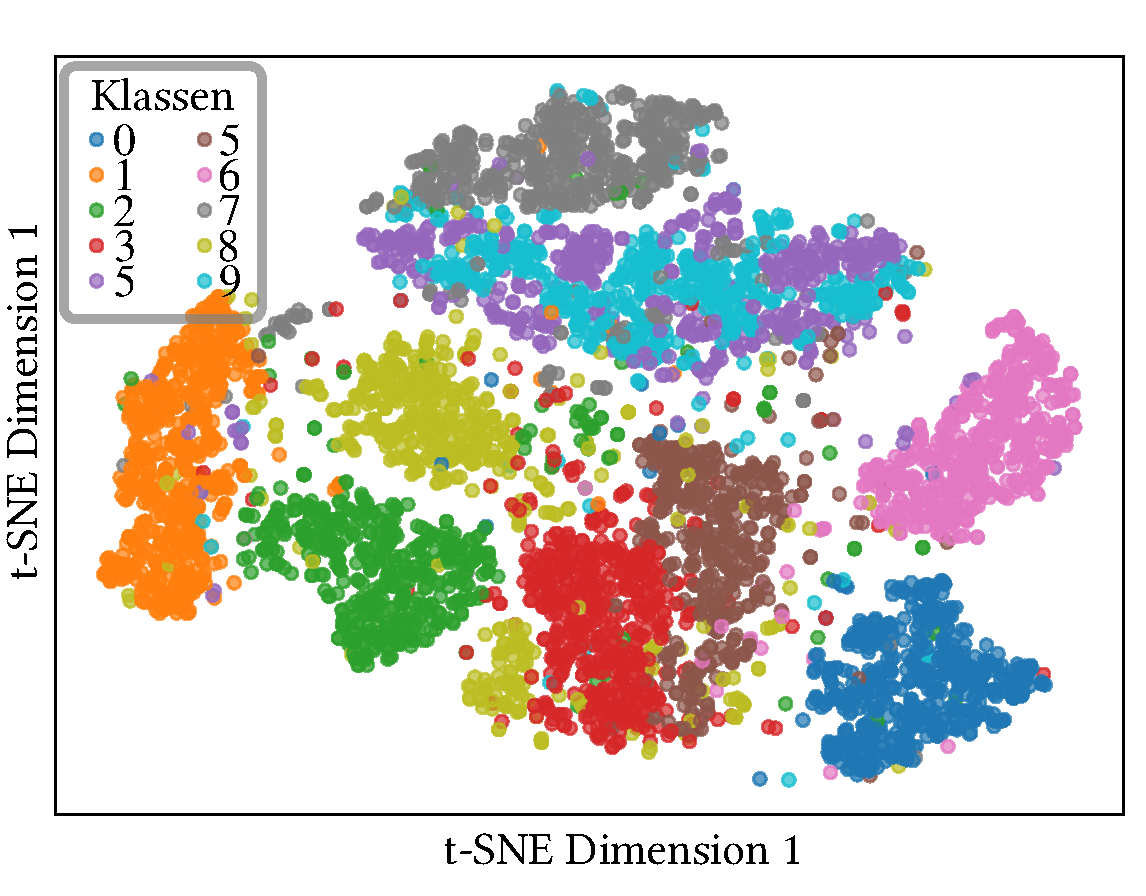
\includegraphics[width=\textwidth]{Figures/scatter_bad.pdf}
        \caption{Epoche 1}
    \end{subfigure} \hfill
    \begin{subfigure}[b]{0.4\textwidth}
        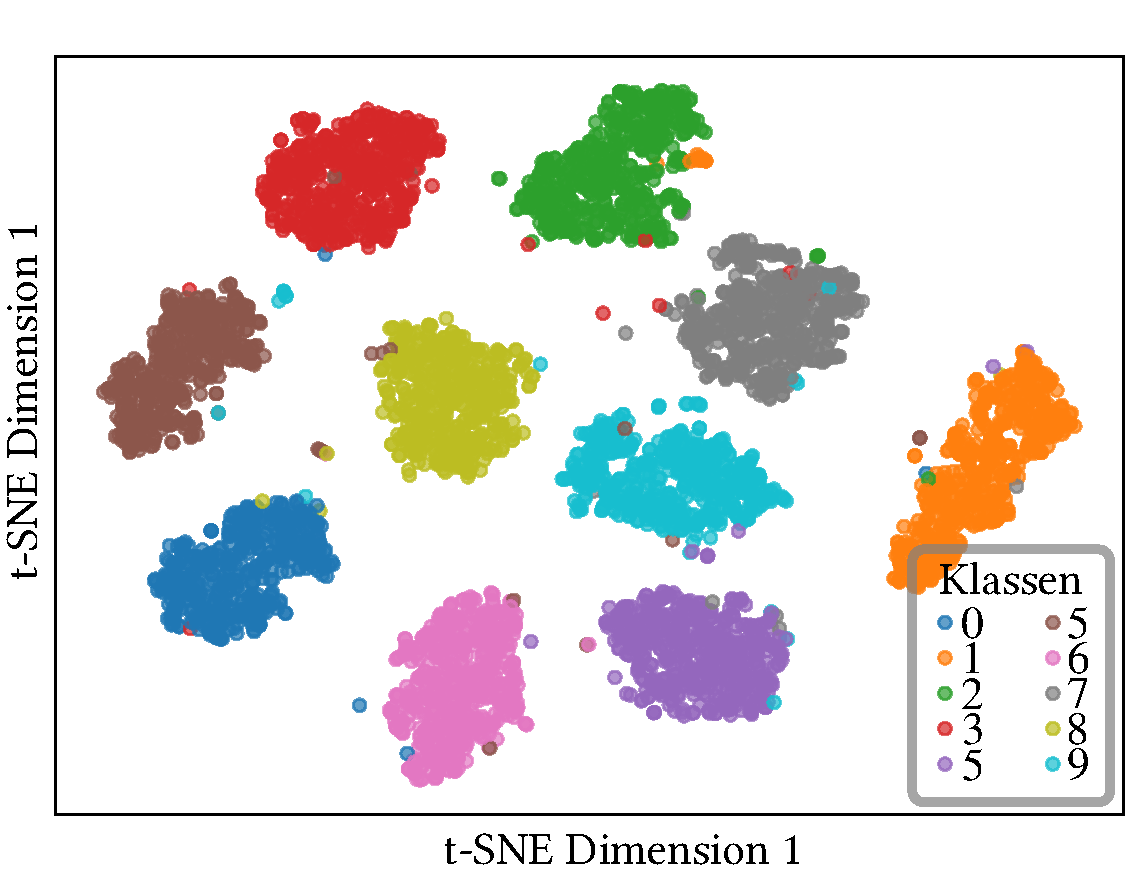
\includegraphics[width=\textwidth]{Figures/scatter_good.pdf}
        \caption{Epoche 25}
    \end{subfigure}
    \caption{Die Abbildung zeigt zwei Scatterplots.
    Beide Scatterplots visualisieren den Merkmalsraum eines Klassifikators, links nach der ersten Epoche des Trainings, rechts nach 25 Epochen.
    Mithilfe der \ac{tsne} ist die hochdimensionale interne Repräsentation der Merkmale in eine zweidimensionale Ansicht projeziert.
    Einige Stichproben des MNIST-Datensatz sind in dieser zweidimensionalen Ansicht platziert und ihre Klassen sind farbig markiert.}
    \label{fig:scatter_tsne_example}
\end{figure}
\textit{TODO: 3D-bzw 2.5D - Welche Methoden werden speziell für 3D-genutzt, gibt es Methoden zur Anpassung?}



\section{Literaturrecherche}

\subsection{Benchmark}\label{sec:bench}
Da das manuelle Erstellen der Annotationen für die Segmentierung von Zelldaten mit erheblichem manuellem Aufwand verbunden ist und zusätzlich Expertenwissen voraussetzt, sind Datensätze hierfür selten. 
Einige prominente Datensätze mit Annotationen für eine Instanzsegmentierung, deren Domänen zu den Zieldaten der Anwendung dieser Arbeit \textit{ähnlich} sind, sind:  
\begin{itemize}
    \item LiveCell \cite{edlund2021livecell}, ein manuell annotierter und Expert*Innen-validierter Datensatz aus 5.239 2D-Bildern. 
    Die Daten sind mit Phasenkontrastmikroskopie gesammelt und enthalten 1.686.352 individuelle Zellen von acht verschiedenen Zelltypen.
    \item YeaZ \cite{dietler2020YeaZ}, ein zweiteiliger Datensatz von Hefe-Zellen aus 87 Phasenkontrast-Bildern mit insgesamt 10.422 Zellen und 614 Hellfeld-Bildern mit insgesamt 3.841 Zellen in 6 Beleuchtungsstufen aufgenommen. Die Annotationen sind semi-manuell erstellt, da die Phasenkontrast-Bilder manuell, und die Lichtfeld-Bilder aus den Phasenkonstrast-Segmentierungsmasken annotiert wurden. 
    \item DeepBas \cite{holden2021deepbacs, cspahn2021deepbacs}, ein Datensatz von \textit{B. subtilis strain SH130} Bakterien. Er besteht aus Weitfeldaufnahmen (Fluoreszenz), aufgenommen mit einem inversen Mikroskop, bestehend aus sieben manuell annotierten Bildern mit je zwischen 46 und 335 Zellen.
    \item die Cell Tracking Challenge \cite{ulman2017cellTrackingChallenge}, eine Sammlung aus 13 Datensätzen verschiedener Mikroskopiemodalitäten, die sich zum Messen der Segmentierungs- und Verfolgungsfähigkeiten für verschiedene Zelltypen eignen.
    \item MoNuSeg \cite{kumar2017MoNuSeg}, eine Zusammenstellung manuell annotierter Gewebeschnitte von sieben verschiedenen Organen. Über 21.000 Zellen sind pro Bild in den 30 Bildern mit verschiedenen Färbungen und Aufnahmetechniken verteilt.
    \item TissueNet \cite{greenwald2022Tissuenet} ein umfassender Datensatz mit über 1.000.000 Zellen mit diversen Gewebearten und unterschiedlichen Aufnahmetechniken.
    \item S-BIAD1518 \cite{Kromp2020_Dataset, chen20223_Dataset}, ein Datensatz der neben manuell annotierten Bildern von acht verschiedenen Zellarten sind synthetisch erzeugte Daten enthält. Mit Hilfe von SpCycleGAN \cite{fu2018cycleGAN} wurden dazu auf Basis von simulierten Annotationen Bildern generiert, die anstreben die Merkmale der realen Bilder zu reproduzieren. Es handelt sich hierbei um 3D-multispektrale Daten, aufgenommen mittels Fluoreszenzbildgebung. 
\end{itemize}
Aufgrund des geringen Volumens frei zugänglicher Daten sind diese Sammlungen auch für das Training von Segmentierungsnetzen begehrt. 
%Jeder Datensatz, der bereits im Trainingssatz eines gewählten Segmentierungsnetzes enthalten war, eignet sich nicht mehr zur unabhängigen Bewertung der Netze. 
Neben annotierten Datensätzen bietet die Literatur auch Methoden zum eigenständigen Erzeugen domänenspezifischer Datensätze \cite{Abay2019, Raghunathan2021, Nikolenko2021, Choi2017, Lu2023}.
Beispielsweise können 3D-Trainingsdaten mit realistischer Zellform und -ausrichtung und umgebenden Markern synthetisch erzeugt und durch ein Generative Adversarial Network an eine gewünschte Bilddomäne angepasst werden \cite{bruch2025}. 
%Das cell synthesis Projekt \cite{bruch2025} ermöglicht das synthetische Generieren von 3D-Trainingsdaten mit realistischer Zellform und -ausrichtung und umgebenden Markern. 
%Zudem umfasst das Framework eine Trainingsroutine, um ein \ac{gan} zu trainieren, das Bilddaten und passende Annotationen automatisch erzeugt und an eine gewünschte Bilddomäne anpasst. 
%
%\begin{itemize}
%    \item \cite{zhu2020domain_similarity} Speech recognition - Herausforderung der Anpassung an Audio domänen
%    \item \cite{han2022binsimilarity_domain} Domain adaption für Bilder (in domain "bins")
%    \item \cite{koohi2018similarity} Maß für Ähnlichkeit in Workflows
%    \item \cite{cai2009similarity} Maß für Ähnlichkeit in Netzwerken
%    \item \cite{wang2018domain}
%    \item \cite{peng2017domain}
%    \item \cite{pinheiro2018domain}
%    \item \cite{ganin2015domain_big}
%    \item \cite{yuan2005domainsimilarity}
%    \item \cite{ganin2016domain}
%\end{itemize}

\subsection{Segmentierungsmodelle}
Foundation-models sind für viele moderne \ac{ki}-Anwendungen unerlässlich \cite{bommasani2021foundationmodels}. 
Sie werden zunächst für allgemeine Aufgaben vortrainiert und anschließend auf spezifische Anwendungen angepasst (fine-tuning), meist unter Einfrieren von Teilen der Gewichte \cite{Yosinski2014}.
Auch Segmentierungsmodelle profitieren stark von umfangreichem Vortraining \cite{dippel2022segmentation}. 
In der aktuellen Forschung werden verschiedene foundation-models für Segmentierung angewandt \cite{wang2021max,zou2023segment,jain2023oneformer,li2023mask}.
Ein prominentes Exemplar ist das \ac{sam} von Meta AI \cite{kirillov2023sam} (siehe Abb. \ref{fig:SAM_Architektur}). 
Es besteht aus einem Bild-Encoder, einem Prompt-Encoder und einem Masken-Decoder. 
\begin{figure}
    \centering
    \includegraphics[width=1\linewidth]{Figures/SAM_Architecture.png}
    \caption{\cite{kirillov2023sam}. Architektur des \ac{sam}. 
    Eingabebilder werden durch einen Bildencoder zu Repräsentationen umgeformt. 
    Zusätzliche optionale Hinweise auf das zu segmentierende Objekt werden durch Bildfaltungen oder einen Prompt Encoder repräsentiert. 
    Anschließend prädiziert der Decoder mehrere mögliche Masken und zugehörige Zuversichtlichkeiten.}
    \label{fig:SAM_Architektur}
\end{figure}
Als Bild-Encoder dient ein Vision Transformer \cite{dosovitskiy2020ViT}, mit Vortraining als Masked Auto Encoder \cite{he2022mae} und zusätzlichem Training für höhere Bildauflösung.
Der Prompt Encoder ist mehrstufig.
Ein angelernter Positional Encoder generiert Repräsentationen aus Positions-Nutzereingaben wie Punkten und Boxen.
Für textuelle Prompts wird der Encoder des CLIP \cite{Radford2021} Models genutzt.
Außerdem werden Bildfaltungen als Encoder auf Masken-Nutzereingaben angewandt.
Mithilfe dieser Encoder wird dem Modell eine Repräsentation von dem zu segmentierenden Bild und optionalen, manuellen Hinweisen auf das erwünschte Ergebnis gegeben, die bereits semantische Informationen und abstrakte Bildmerkmale beinhalten.
Aus diesen Repräsentationen generiert dann der Decoder mehrere mögliche Masken mit zugehörigen Zuversichtlichkeiten, aus denen ein finales Segmentierungsergebnis ausgewählt wird.\newline
\ac{sam} wurde bereits für viele explizite Mikroskopie-Zelldaten Anwendungen angepasst \cite{archit2025samfine, israel2023samfine, vandeloo2025samfine}. 
Auch für bestehende biologische Segmentierungsanwendungen, wie etwa Cellpose\cite{stringer2021cellpose}, wurde \ac{sam} auf Zelldaten angepasst \cite{pachitariu2025samcellpose}.
Dieser \textit{Fine-tune} nennt sich CellposeSAM.
Er kombiniert den Bild-Encoder von \ac{sam} mit dem \textit{Flow}-Segmentierungsansatz von Cellpose.
Dabei generiert der Bild-Encoder direkt Vekotoren, die Zwischenrepräsentationen, die sogenannten \textit{Flows}, darstellen.
Diese \textit{Flows} werden pixelweise zu einem Gradientenfeld überführt.
Mithilfe der Gradienten werden Objektinstanzen vorhergesagt.
Abb. \ref{fig:CellposeSAM} zeigt diesen Ablauf als Diagramm. \newline
\begin{figure}
    \centering
    \includegraphics[width=1\linewidth]{Figures/CellposeSAM_Diagramm.png}
    \caption{Ablauf des CellposeSAM-Modells. 
    Eingabebilder werden durch einen Bild-Encoder (ViT-L) direkt zu sogenannten \textit{Flows} umgeformt, einer Repräsentation von vorhergesagten Objektmerkmalen, deren Wert von der relativen Position innerhalb des detektierten Objekts abhängt. 
    Die Gradienten der Flows werden verfolgt (gradient tracking) und aus dem daraus entstehenden Gradientenfeld werden Segmentierungsinstanzen (ROIs) vorhergesagt \cite{pachitariu2025samcellpose}.}
    \label{fig:CellposeSAM}
\end{figure}
Deepcell \cite{van2016deepcell,bannon2021deepcell,greenwald2022deepcell} bietet weitere Zellsegmentierungsmodelle.
Das Deepcell-Caliban-Modell \cite{moen2019DeepcellCaliban} nutzt als Encoder eine EfficientNetV2L-Architektur \cite{Tan2021}, an deren Ausgabeschichten (C1\–C5) eine Pyramiden-Struktur zur Merkmalsfusion (P1\–P7) angeschlossen ist. 
Eine Besonderheit des Netzes ist, dass Eingabebildern zusätzlich Koordinatenkarten hinzugefügt werden.
Als Decoder dienen drei Segmentierungsköpfe, die verschiedene Transformationen der gelabelten Trainingsmasken vorhersagen.\newline
In der Literatur sehr verbreitet ist außerdem das nnU-Net \cite{isensee2021nnu}, ein Segmentierungsframework, das sich automatisch an neue biomedizinische Aufgaben anpasst.
Es konfiguriert Vorverarbeitung, Netzwerkarchitektur, Training und Nachbearbeitung dynamisch auf Basis der Eigenschaften des jeweiligen Datensatzes. 
Die Leistungsfähigkeit des Ansatzes ergibt sich nicht aus einer neuen Architektur oder Lernmethode, sondern aus der konsequenten Automatisierung und Systematisierung von Entwurfsentscheidungen.

\subsection{Klassifikator}
%\textbf{QUELLEN NOCH!}\newline
Für Klassifikatoren werden in der Regel nur Encoder vortrainiert, der Klassifikations-Kopf muss an die Klassen des vorliegenden Problems angepasst werden \cite{Plested2022, Yosinski2014, Dippel2022}.
State-of-the-Art für Bild-Encoder sind \acp{cnn} oder \acp{vit}, die auf dem ImageNet \cite{Russakovsky2015} Datensatz vortrainiert werden \cite{You2018, Kornblith2019}.
Klassifikatoren profitieren stark von ImageNet-Vortraining \cite{Beyer2020, Recht2019}.\newline
\textbf{ResNet} ist ein Residual Neural Network, ein \ac{cnn} mit sogenannten residual connections \cite{He2016}.
Diese residual connections verbinden den Ein- und Ausgang modularer Faltungsschichten und verbessern die Leistungsfähigkeit tiefer neuronaler Netze \cite{He2015, He2016, srivastava2015highway} (siehe Abb. \ref{fig:ResCon}).
%\begin{figure}
%    \centering
%    \includegraphics[width=0.4\textwidth]{Figures/ResidualConns.png}
%    \caption{Residual connection. Der Eingang des modularen Blocks ist mit dem Eingang direkt verbunden \cite{He2016}.}
%    \label{fig:ResCon}
%\end{figure}
In ihrem Paper stellen die Autoren fünf unterschiedlich tiefe Varianten der \textbf{ResNet}-Architektur vor.
Jede Variante enthält fünf Blöcke mit residual connections.
Die Blöcke bestehen aus Faltungen mit verschiedenen Kernelgrößen und Strides, Batch normalization \cite{Ioffe2017} und der ReLU \cite{Nair2010} Aktivierungsfunktion.\newline
\textbf{EfficientNetV2} ist ein Nachfolger der EfficientNet-Modellfamilie \cite{Tan2019, Tan2021}.
Die Architektur basiert auf modularen Blöcken von Bildfaltungsoperatoren mit besonders kleinen Faltungskernen und Squeeze-and-Excitations, genannt MBConv \cite{Sandler2018, Tan2019} und Fused-MBConv \cite{Gupta2019} (siehe Abb. \ref{fig:MBConv}).\newline
%einer Kombination aus MBConv- \cite{Sandler2018, Tan2019} und Fused-MBConv-Blöcken \cite{Gupta2019}, also aus .
%Beide MBConv-Arten nutzen dabei Squeeze-and-Excitation und 1x1-Faltungsschichten.
%Während MBConv aber die Dimension der Daten mithilfe einer weiteren 1x1 Faltung und 3x3 Depthwise-Faltung erhöht, nutzt der Fused-MBConv-Block hierzu eine reguläre 3x3 Faltung 
\begin{figure}[htbp]
    \centering
    \begin{subfigure}[b]{0.48\textwidth}
        \includegraphics[width=1\textwidth]{Figures/ResidualConns.png}
        \caption{Residual connection. Der Eingang des modularen Blocks ist mit dem Eingang direkt verbunden \cite{He2016}.}
        \label{fig:ResCon}
    \end{subfigure} \hfill
    \begin{subfigure}[b]{0.48\textwidth}
        \includegraphics[width=1\textwidth]{Figures/MBConv.png}
        \caption{MBConv- und Fused-MBConv-Blöcke. Die Blöcke nutzen neben einer residual connection auch Faltungsschichten und Squeeze-and-Excitation, um die Datendimension zu erhöhen \cite{Tan2021}.}
        \label{fig:MBConv}
    \end{subfigure}
    \caption{Diagramme a) der Residual Connections und b) MBConv-Blöcke und Fused-MBConv-Blöcke.}
    \label{fig:ResDiagramms}
\end{figure}
\textbf{ConvNeXt} \cite{Liu2022} ist eine \ac{cnn}-Modellfamilie mit besonders großen Faltungskernen. 
Die \textbf{ConvNeXt}-Architektur umfasst fünf modulare Blöcke mit Faltungen und residual connections, wie die ResNet-Architektur \cite{He2016}.
Allerdings verändert dabei \textbf{ConvNeXt} einige Details der ResNet Architektur, wie beispielsweise die GeLU Aktivierungsfunktion \cite{Hendrycks2016} und Layer normalization \cite{Ba2016}.\newline
Swin Transformer \cite{liu2021} ist eine beliebte Modellfamilie von \acp{vit}.
Ihr Nachfolger, die \textbf{Swin Transformer V2} \cite{Liu2022a}, vergrößert die Modelle noch.
Die Architektur kombiniert Bildausschnitte mit einem Positions-Bias.
Hierzu werden ein Bildfenster $z$ und dessen relativen Koordinaten im Bild $\Delta x$ und $\Delta y$ in einem Attention-Mechanismus zusammengeführt.
Die Positionen werden in einem MLP-Netz verarbeitet, während das Bildfenster mit drei verschiedenen Gewichtsmatrizen multipliziert wird.
Mithilfe einer Kosinus-Ähnlichkeitsfunktion, der Softmax-Funktion \cite{Bridle1989} und elementweiser Multiplikation sowie Addition werden diese Ergebnisse in einen Merkmalsraum überführt.
Zwei Layer normalization \cite{Ba2016} Schichten, ein weiteres MLP-Netz und residual connections vervollständigen anschließend den modularen \textbf{Swin Transformer V2} Block.
Dieser Aufbau ist in Abb. \ref{fig:SwinArchitecture} dargestellt. 

%Backbones:
%\cite{He2016} ResNet
%\cite{Tan2021} EfficientNetV2L
%\cite{Liu2022} convnextxl
%\cite{Liu2022a} SwinV2

\section{Offene Probleme}
Einzelne Myotuben können durch kein Segmentierungsmodell der Literatur instanzsegmentiert werden.
Selbst für Expert*Innen sind in dichten Strukturen Instanzen von Myotuben nicht immer eindeutig trennbar.
%Es ist nicht erforscht, welches Segmentierungsmodell für Nuclei das beste ist, im Bezug auf die Eignung der Segmentierungsmasken zur Extraktion von Eigenschaften der Nuclei.
Nicht viele Segmentierungsmodelle für Nuclei sind erhältlich, besonders für dreidimensionale Daten.
Die verfügbaren Modelle verhalten sich unterschiedlich bei verschiedenen Datensätzen und ihre Eignung für bestimmte Aufgaben muss für jede Anwendung individuell geprüft werden.
Die Daten der vorliegenden Arbeit sind nach dem Protokoll in Couturier et al., \cite{Couturier2024} erstellt und umfassen Myotubenkulturen und ihre Nuclei mit insgesamt fünf verschiedenen Fluoreszenzmarkern.
Für die spezifischen Aufnahmebedingungen und Marker der vorliegenden Daten gibt es keinen angepassten Klassifikator.
Der Erfolg von einem Übertrag verschiedener vortrainierter Encoder und etablierter Methoden auf die vorliegenden Daten ist unvorhersehbar, da sich die gelernten Merkmalsräume eventuell nicht für die Klassifikation der neuartigen dreidimensionalen Daten eignen.
Eine weitere Fragestellung ist deshlab, wie Methoden der Klassifikation mit der Kombination der Marker umgehen. 
Für jeden Datensatz mit neuen Zellkernklassen und Aufnahmebedingungen muss für optimale Klassifikatorleistung nicht nur ein neues Modell trainiert werden, sondern auch Methoden- und Hyperparameteroptimierung durchgeführt werden.
Des Weiteren ist der Umgang mit dreidimensionalen Daten, besonders in Umgebungen ohne große Rechenleistung ein offenes Problem.
Diverse Lösungen existieren, um dreidimensionale Daten mit Expertenwissen zu versehen.
Diesen Lösungen fehlt bislang, ein Arbeitsablauf der Daten unmittelbar segmentiert und vorbereitet, um relevante Bildausschnitte direkt aus dem Datensatz zu extrahieren, sodass Expert*Innen ausschließlich annotieren müssen.

\section{Zielsetzung}
Im Zuge der vorliegenden Arbeit soll die automatische Extraktion von interpretierbaren Eigenschaften der Myotubenkulturen ermöglicht werden.
Zu diesem Ziel bearbeitet die vorliegende Arbeit Zwischenziele und liefert Folgendes:
\begin{itemize}
    \item Es soll ein Segmentierungsmodell gefunden werden, das die Eigenschaften der Nuclei in den vorliegenden, dreidimensionalen Daten besonders wenig durch Segmentierungsfehler verfälscht.
    Dazu wird ein neues Bewertungskriterium für Instanzsegmentierung eingeführt und auf einige etablierte Modelle angewandt.
    \item Das Segmentierungsmodell soll dann genutzt werden, um außerdem einen Ablauf zu schaffen, in dem Expert*Innen die Klassen der Nuclei besonders zeiteffizient annotieren können, um einen Klassifikator zu trainieren.
    Durch das Anreichern der dreidimensionalen Daten durch die Segmentierungsmasken und durch automatisches Fokusieren einzelner Nuclei soll sowohl die Rechenzeit optimiert werden als auch der Aufwand einzelne Nuclei entlang drei Dimensionen zu suchen, eliminiert werden.
    Hierzu wird eine neue Anwendung entwickelt, die 3D-Zelldaten liest und dann eine Oberfläche zum Annotieren bereitstellt.
    \item Die enstehenden Annotationen sollen direkt in einen Trainingsablauf für Klassifikatoren eingebunden sein.
    Hierbei müssen Klassifikatoren mit dreidimensionalen Daten von variierender Tiefe umgehen können.
    Ein ausführlicher Methodenvergleich verschiedener Encoder, Klassifikations-Köpfe, Vorverarbeitungsmethoden und auch Vortrainingsmethoden soll für Nutzer*Innen ohne Programmierkenntnisse ermöglicht werden.
    Dazu wird eine neue Anwendung entwickelt, die die zuvor erstellten Annotationen und Segmentierungsmasken nutzt um einen Klassifikator zu trainieren.
    Nutzer*Innen können in einer grafischen Oberfläche verschiedene Methoden zum Vergleich auswählen und in einem automatischen Prozess werden Klassifikatoren aller Kombinationen trainiert und verglichen.
    \item Außerdem sollen die ausgelesenen Eigenschaften der eingegebenen Zelldaten leicht zugänglich sein.
    In einer weiteren neuen Anwendung werden automatisch die Vorhersagen des Klassifikators mit dem besten Ergebnis im Methodenvergleich genutzt, um Nutzer*Innen Graphen mit den Eigenschaften der Zellkultur darzubierten.
    \item Zuletzt sollen alle neu entwickelten Module zu einer Gesamtanwendung zusammengefasst und getestet werden.
    In einer Parameterbestimmung wird das Optimum explizit für die vorliegenden Aufnahmen mithilfe der neuen Anwendung bestimmt.
\end{itemize}

%Die Positionen und Klassen der Nuclei sollen dann codiert werden, um die Daten damit Anzureichern und dadurch einem Segmentierungsmodell die Instanzsegmentierung der Myotuben zu ermöglichen. 